\documentclass[11pt]{article}

\usepackage[a5paper,left=2cm,right=1cm,top=1cm, bottom=1.5cm]{geometry}
\usepackage{array}
\usepackage{makecell}
\usepackage[all]{nowidow}
\usepackage{wrapfig}
\usepackage{enumitem}
\usepackage{multicol}

\usepackage{hyperref}
\hypersetup{
    colorlinks=true,
    urlcolor=sokolblue,
    }

\usepackage[czech]{babel}
\usepackage[utf8]{inputenc} 
\usepackage{ellipsis}

\usepackage{fontspec}
\newfontfamily{\tyrs}{Sokol Tyrs}
\newfontfamily{\fugner}{Sokol Fugner}

% \usepackage{lmodern}
% \usepackage[T1]{fontenc} 
\usepackage{anyfontsize}
\newcommand{\titlesize}{\fontsize{56pt}{67pt}}


\usepackage[dvipsnames]{xcolor}
\definecolor{sokolred}{RGB}{228, 5, 33}
\definecolor{sokoldarkred}{RGB}{200, 0, 30}
\definecolor{sokolblue}{RGB}{45, 46, 135}

\usepackage{tikz}
\usetikzlibrary{calc}

\usepackage{fancyhdr}

\fancypagestyle{standard}{%
    \fancyhf{}
    \fancyhead[LO]{%
        \begin{tikzpicture}[overlay,remember picture]
            \fill [color=sokolred] (current page.north west) rectangle ($ (current page.south west) + (1cm,0cm) $);
            \fill [color=sokolred] ($ (current page.north west) + (1.1cm,0cm) $) rectangle ($ (current page.south west) + (1.2cm,0cm) $);
        \end{tikzpicture}
        }
    % \fancyhead[RE]{%
    %     \begin{tikzpicture}[overlay,remember picture]
    %         \fill [color=orange](current page.north east) rectangle
    %             ($ (current page.south east) + (-1cm,0cm) $);
    %     \end{tikzpicture}
    %     }
    \fancyfoot[C]{%
      \begin{tikzpicture}[overlay,remember picture]
        \fill [color=sokolred] ($ (current page.south east) + (-1.5cm,1.3cm) $) rectangle ($ (current page.south east) + (0cm,0.5cm) $)
         node [pos=0.5,color=white] {\large\tyrs{\thepage}\hspace*{0.5cm}};
      \end{tikzpicture}
    }

    \renewcommand{\headrulewidth}{0pt}
    \renewcommand{\footrulewidth}{0pt}
}



\fancypagestyle{uvodnik}{%
    \fancyhf{}
    \fancyfoot[C]{%
      \begin{tikzpicture}[overlay,remember picture]
        \fill [color=sokolred] ($ (current page.south east) + (-1.5cm,1.3cm) $) rectangle ($ (current page.south east) + (0cm,0.5cm) $)
         node [pos=0.5,color=white] {\large\tyrs{\thepage}\hspace*{0.5cm}};
      \end{tikzpicture}
    }

    \renewcommand{\headrulewidth}{0pt}
    \renewcommand{\footrulewidth}{0pt}
}

\fancypagestyle{blank}{%
    \fancyhf{}
    \fancyfoot[C]{}

    \renewcommand{\headrulewidth}{0pt}
    \renewcommand{\footrulewidth}{0pt}
}


\newcommand{\post}[1]{%
\begin{center}
{\huge \tyrs #1}
\end{center}
}

\newcommand{\subpost}[1]{%
\vspace*{12pt}
\begin{center}
{\Large \tyrs #1}
\end{center}}

\newcommand{\signature}[2]{%
  \begin{flushright}
    \textbf{#1}\\#2
  \end{flushright}
}

\newcommand{\luv}{\clqq\kern-0.07em}
\newcommand{\ruv}{\kern0.07em\crqq\kern0.1em}

\usepackage{csquotes}
\DeclareQuoteAlias{german}{czech}
\MakeOuterQuote{"}

\usepackage[normalem]{ulem}



\babelhyphenation{Ra-kou-ska-Uher-ska}
\begin{document}

%% title
\newgeometry{margin=1cm}
\pagecolor{sokolred}
\color{white}
\pagenumbering{gobble}
\begin{center}

\vspace*{\fill}

{\titlesize \fugner ZPRÁVY}

{\titlesize \tyrs SOKOLA LIBEŇ}

\vspace*{1cm}

{\large ročník LI · číslo 3 · květen 2025}

\vspace*{\fill}
\end{center}

\clearpage
\normalcolor
\nopagecolor
\pagenumbering{arabic}

%% úvodník
\pagestyle{uvodnik}
\newgeometry{margin=1.5cm}

\setlength{\columnsep}{-2.5cm}
\begin{multicols}{2}
  {\fontsize{48pt}{57pt} \fugner \color{sokolred} \noindent Úvodník}

  \columnbreak

  \vspace*{-4pt}

  {\hfill\textbf{Vít Jakoubek}}
  
  % {\hfill\textbf{Místonáčelník}}
 \end{multicols}

\vspace*{12pt}

\noindent
Milé sestry, milí bratři, vážení příznivci Sokola Libeň!

\noindent
Jsme téměř v~polovině roku, ve kterém se konala a ještě bude konat řada
voleb, a to nejen na podzim do Poslanecké sněmovny. 19. března se konala
Valná hromada naší jednoty, na které byl zvolen nový výbor pro další
tříleté volební období ve složení:

\vspace*{12pt}

starosta: Jiří Novák,

jednatel: Jan Přech,

místostarostka: Drahomíra Černičková,

vzdělavatelka: Anna Holanová,

členka výboru: Dana Cejpková,

člen výboru: Jiří Duchač,

členka výboru: Dáša Francková,

člen výboru: Vít Jakoubek,

člen výboru: Jan Přibyl.

\vspace*{12pt}

Náhradníky výboru pak byli zvoleni: Lucie Vojáčková, Jan Kerhart,
Vladislav Voráč a Jakub Jabor.

Valná hromada dále zvolila Kontrolní komisi ve složení: Pavel Lávička,
Tomáš Troup a Hana Doupalová; náhradníkem byl zvolen Miloslav Doupal.

Valná hromada pak také vzala na vědomí zvolení náčelnictva, které si
volí jednotlivé cvičitelské sbory: náčelníka ženských složek Tomáše
Dragouna a náčelníka mužských složek Josefa Kubištu. Tito se automaticky
stávají členy výboru. Do funkce starosty ČOS pak Valná hromada navrhla
našeho člena a cvičitele Martina Chlumského, který již nyní tuto funkci
zastává.

Valná hromada proběhla rovněž v~naší župě Jana Podlipného: do funkce
starosty župy byl zvolen Martin Chlumský, náčelnicí Dagmar Fischerová a
náčelníkem Petr Čížkovský.

V~červnu se pak bude konat Sjezd ČOS, na kterém bude zvolen nový Výbor
ČOS, starosta a jednatel.

Župní náčelnice již zvolily náčelnicí ČOS Kateřinu Machů (Sokol Praha
Vršovice) a župní náčelníci zvolili náčelníkem ČOS Petra Sádka (Sokol
Turnov). Vzdělavatelský odbor ČOS zvolil vzdělavatelem ČOS Michala
Buriana a valná hromada Odboru sportu ČOS zvolila svým předsedou Jana
Haupta.

Jistě jsme všichni zaznamenali velmi turbulentní události, které se
udály v~ústředí naší organizace. Celá záležitost ještě není uzavřena,
ale volba nového Výboru ČOS jí jistě bude ovlivněna.

Přejme si, aby byli zvoleni ti, kteří to s~naším spolkem myslí dobře.
Aby byli zvoleni ti, kteří nemyslí jen na sebe, nýbrž na ty, kteří je
volili, ale i na ty, kteří je nevolili. Přejme si, aby byli zvoleni ti,
kteří mají pevný charakter, plní své slovo a kteří dokáží myslet dále
než do konce aktuálního volebního období. Takových nám bude zejména
v~dnešní době více než třeba. A~osobně si přeji, aby právě takoví lidé
byli zvoleni i v~podzimních volbách do Poslanecké sněmovny PČR.

Jako editor těchto Zpráv bych vás všechny také rád požádal o~spolupráci
při tvorbě jejich obsahu:

Pokud byste měli nějaké náměty, o~čem by se mělo psát, pak mi o~tom
prosím dejte vědět.

Pokud byste také sami rádi něco napsali, pak se neostýchejte a text mi
pošlete: bude velmi cenné číst texty jiné než jen od činovníků. Ostatně,
minulé mimořádné historické číslo bylo důkazem, že do Zpráv velmi hojně
psali právě běžní členové, dospělí i nezletilí. Prosím, nechte se jimi
inspirovat, bude to pro všechny jistě obohacující.

\vspace*{12pt}
\noindent
Nazdar!
\clearpage

%% termínka

\pagecolor{sokolred}
\color{white}
\renewcommand{\arraystretch}{1.2}

\newcommand{\boxheight}{11.7cm}

\vspace*{\fill}
\post{TERMÍNOVÁ LISTINA AKCÍ JEDNOTY}
\vspace*{0pt}

\begin{center}
\begin{tikzpicture}
  \draw [ultra thick,color=white](0.3cm,0cm) rectangle (12.3cm,\boxheight);
  \fill [color=white] (0cm,0.3cm) rectangle (12cm,\boxheight + 0.3cm)
  node [pos=.5, color=black] {
    \begin{tabular}{l  p{6.5cm}}
      29. 5. (čt) & Dětský den a loutkové představení (16:30--19:00) \\
      30. 5.--1. 6. (pá--ne) & Finále ČOS ve všestrannosti ml. žactva \\
      30. 5.--1. 6. (pá--ne) & příprava nového tábořiště v~Keblanech \\
      8. 6. (ne) & atletické závody rodičů a děti, předškolních dětí a nejml. žactva \\
      6.--8. 6. (pá--ne) & Finále ČOS ve všestrannosti st. žactva \\
      20.--22. 6. (pá--ne) & Stěhování tábora Velhartice–Keblany \\
      27.--29. 6. (pá--ne) & Stavba tábora \\
      26. 6. (čt) & Zakončovací táborák \\
      27. 6. -- 19. 7. & tábor oddílu Veverky a JILM \\
      5.--12. 7. & tábor oddílu Venkovních sportů -- Janské Lázně \\
      12.--19. 7. & pobyt rodičů a dětí -- Janské Lázně \\
      19.--26. 7. & tábor bývalých členů JILMu \\
      26. 7. -- 9. 8. & tábor oddílu Káňata \\
      8.--10. 8. (pá--ne) & Bourání tábora \\
      1. 9. (po) & začátek cvičení po prázdninách \\
      25. 9. (čt) & Běh strmý \\
    \end{tabular}
  };
  %  node [color=black] {FOOBAR};
\end{tikzpicture}

\renewcommand{\arraystretch}{1}

\vspace*{12pt}
Podrobné informace k~akcím budou zveřejňovány na našich internetových stránkách a distribuovány dalšími obvyklými kanály (cvičitelé, vývěsky, e-mail)

\end{center}
\vspace*{\fill}

\clearpage
\nopagecolor
\normalcolor

%% normální obsah
\restoregeometry
\pagestyle{standard}

\post{Zpráva o~dění ve cvičení žáků a v~celé jednotě}

Od posledních Zpráv, které vyšly koncem února, jsme se ve cvičení
nezastavili.
Zimní soutěž, nominační závody, běžné cvičení, nácvik závodních sestav
s~vybranými kluky a nakonec i závody všestrannosti. Nakonec se vše
zvládlo
a výsledky snažení snad nakonec stály za to. A~teď tedy postupně o~tom
jarním ruchu.
Pokračovala Zimní soutěž žáků v~házení, kopání a střelbě míčků
do malé
florbalové branky.
11. a 13.~2.~2025 se konaly Nominační závody žáků. Gymnastické
sestavy
na kruzích, hrazdě, bradlech, přeskok, prostná a šplh si zkusilo 92
kluků (46
mladších žáků, 40 starších žáků a 6 dorostenců). Celkem jsme vybrali 32
kluků pro další nácvik na dubnové závody všestrannosti. Po různých
omluvách, nemocech a zraněních nám v~nácviku zbylo 21 žáků.

\subpost{Závody a soutěže}
Celopražské Závody všestrannosti proběhly v~termínu 25.--27. 4.
2025.
Dle vypsaných kategorií jsme vyslali 11 mladších žáků, 8 starších žáků,
2
dorostence a 5 mužů. Celkem tedy 26 cvičenců. A~protože se v~žácích
účastnilo celkem 39 závodníků z~naší župy, měli kluci jen 20 soupeřů a
možnost mnoha dobrých umístění. V~jednotlivých disciplínách (plavání,
gymnastika, šplh a atletika) jsme získali 27 medailových umístění,
o~které se
rozdělilo 12 z~19 našich žáků. V~celém čtyřboji byl J. Vandas a H.
Höschl 1., L. Bednář a J. Doupal 2. (a všichni 4 postupují na celostátní
finále) a A. Příhoda a M. Sokol 3., 4. místo obsadili M. Cakl a Š.
Novák, 5. F. Vikler a J. Šefrna.
Děkujeme všem závodníkům za pěkné výkony a rodičům za trpělivost při
nácviku i při závodech.
Kromě závodníků jsme museli na závody samozřejmě vyslat i doprovázející
cvičitele a rozhodčí -- celkem to bylo 12 cvičitelů.
Ve středu 8. května se konal gymnastický závod Praha Open
(společný
pražský závod pro Sokol a Asociaci sportu pro všechny), kam ze závodu
všestrannosti postoupilo 14 našich žáků. Devět se jich závodu zúčastnilo
a
vedlo si výsledkově o~něco hůře než na župních závodech. Kromě toho
závodil ve všestrannosti i jeden muž.
Trvá celoroční soutěž O~nejvěrnější docházku s~pravidelným
každoměsíčním vyhlašováním a rozdáváním diplomků za 100\% docházku.

\subpost{Organizační informace}
Cvičení venku s~atletickými disciplínami začalo 29. dubna a za dobrého
počasí bude pokračovat do konce června. V~případě velké zimy nebo deště
cvičení v~sokolovně. I~ven se nosí jako úbor bílé tričko se znakem a
modré
trenky a vhodná sportovní obuv -- žádné tepláky a bundy nejsou při
cvičení
potřeba, dostatečně se zahřejeme pohybem. Začátek i konec hodiny v~šatně
-- děkujeme!
Letošní docházka je zatím velmi početná. Nejnižší průměr od
září 2024
byl v~prosinci -- 54,0. Nejvyšší průměry byly v~listopadu -- 66,75 a
dubnu
65,25, což byly zároveň měsíce, kdy mělo nejvíce kluků 100\% docházku --
24, respektive 21. Každý měsíc je zapsáno přes 100 žáků. Tak ať nám tato
krásná čísla vydrží ve zbytku jara a zůstanou i na podzim.

\subpost{Brigáda}
V~neděli 2. března proběhla tradiční Jarní brigáda v~sokolovně a okolí.
Ruku k~dílu přiložilo 15 cvičitelů, 3 cvičitelky, 7 žáků, 5 žákyň, 7
Jilmáků, 1
Veverka, 8 mužů, 1 žena, 6 rodičů a 2 děti. Celkem tedy 55 lidí.
Venku se umístily obrubníky kolem tahací dráhy a zryla a urovnala hlína
pro
zamýšlený trávník za sokolovnou. Za pomoci příklepových vrtaček se
sejmul
obklad z~nové podzemní místnosti (požadavek památkářů) a \uv{napytloval}
se
do vodáckých barelů k~pondělnímu odvozu do sběrného dvora. Hrabalo se
listí
na trávníku a před kostelem, zametl se chodník ke gymnáziu. Za
sokolovnou
se podařilo dodláždit polovinu pruhu bez kostek, ostatní kostky se
přerovnaly
na nové místo. Svařilo se kolečko a florbalové branky.
V~sokolovně probíhala spousta drobnějších prací: umyly se všechny
žíněnky, míče, tyče, florbalky, desky košů, utřel se prach v~šatnách a
na reproduktorech v~sále, umyly se
botníky, v~sále se odstranily poslední modré značky ze sletu, opravilo
se
obložení radiátorů a stálky, vysál gymnastický koberec, natáhly se sítě
na
nové florbalové branky, natřely jedny dveře za šatnou mužů, upevnily se
všechny kliky v~sálech, opravil šuplík skříně Srncova sálu, namontovala
se
časomíra pro měření šplhu, podlepilo se veškeré přeskokové nářadí,
vysálo
se ve Filipově síni a proběhly i další drobné a úklidové práce.
Odpracováno bylo mezi 9. ranní a 16. odpolední 288 hodin. Děkuji všem
zúčastněným a slibuji, že na podzim bude práce stále dosti. A~aby se nám
nezkrátily žíly, bude se o~prázdninách předlážďovat historická dlažba za
sokolovnou -- vytrháme kostky, podsypeme štěrkem a krásně uložíme zpět
do trochu vyšší pozice. Tím se nám vyprázdní uhelna od tam uskladněného
štěrku, abychom do ní mohli následně umístit nádrže na dešťovou vodu (na
zalévání našich trávníků).

\subpost{Šibřinky}
V~sobotu 8. 3. 2025 byly na programu tradiční Šibřinky. Ráno se vše
připravilo. Vyklidil se sál, přerovnalo nářadí, nanosily stoly a židle,
pódia
pro kapelu, nainstalovala se rozsáhlá výzdoba sálu, připravil se bar,
skříně se
sklenicemi, zapojil dřez pro mytí nádobí a provedly se další drobné
práce.
Přišlo 28 pomocníků, kterým vše trvalo necelé 2 hodiny. Pak rychle na
oběd
a v~15:00 začaly Dětské šibřinky ve stylu Pejsek a kočička, na které
dorazilo asi 75 dětí v~maskách. Na programu byly tanečky, masky,
vystoupení Tomáše Dragouna s~žonglovacími míčky a v~druhé části pak
bylo připraveno 9 soutěží inspirovaných příhodami dvou výše zmíněných
postaviček, po nichž byli úspěšní účastníci obdarováni drobnou odměnou.
Díky všem 32 pomocníkům, kteří se postarali o~hladký průběh akce. Okolo
páté odpolední byly děti odeslány domů, aby rodiče a další zájemci mohli
o~sedmé večerní dorazit na Šibřinky pro dospělé s~podtitulem Cirkus. Byla
živá kapela, tombola, soutěž masek, občerstvení, předtančení
československá (sokolská) beseda a irské tance, ukázka akrojógy. Přišlo
asi 110 účastníků, kteří se dobře bavili.
Děkujeme všem 25 osobám, které držely na večerních Šibřinkách služby
(snos a mytí nádobí, prodej občerstvení, obsluha na baru, výčep piva).
Zvláště pak děkujeme starším sestrám, které napekly spoustu výborných
dobrot pro děti i pro dospělé.
V~neděli pak 17 ochotných vytrvalců mezi 10. a 14. vše vzorně uklidilo.

\subpost{Valná hromada}
Ve středu 19. 3. 2025 se konala Valná hromada Sokola Libeň. K~17. 3.
měla naše jednota 783 členů (157 předškolních dětí, 142 žáků, 129 žákyň,
163 mužů a 192 žen), které na valné hromadě zastupovalo 41 delegátů z~44
zvolených. Na valné hromadě byla schválena výroční zpráva za rok 2024,
zpráva kontrolní komise a rozpočet jednoty na rok 2025 ve výši 7 320 000
Kč. Dále se probraly věci cvičební i k~provozu sokolovny za rok 2024 a
přednesl se výhled činnosti na rok 2025. Valná hromada též zvolila
\uv{nový}
výbor a kontrolní komisi na další tříleté funkční období, a to ve
stejném
složení, v~jakém dosud pracovaly.
V~pondělí 14. 4. proběhla valná hromada župy. Župním starostou
byl zvolen
Martin Chlumský -- Čedok. Náčelníkem a náčelnicí zůstávají Petr
Čížkovský a
Dagmar Fischerová.

\subpost{Jarní Výlet Libeňského Sokola}
V~sobotu 12. 4. se 64 Libeňáků sešlo na 68. Jarním Výletě Libeňského
Sokola. Spolu s~jednotami ze Starého Města, Proseka, Prahy 7 a Zlíchova
jsme byli účastníky 59. srazu v~přírodě pražských žup. Celkem nás bylo
127.
Vlakem jsme vyrazili z~hlavního nádraží do Malé Hraštice a pak skoro 5
km
pěšky přes pole, okolo Velké Hraštice do Velké Lečice a pak k~Malé
Lečici
k~vodopádku Kocáby, kde v~jezírku proběhla Modrá stuha. Díky letošnímu
chladnému počasí měla voda jen 10,5 °C. Po nástupu s~Písničkou,
Jazykohrátkami a Pamatovačkou jsme se rozdělili na dvě hlavní části --
účastníky a organizátory župního přeboru v~Zálesáckém závodu zdatnosti
(ZZZ) a zbytek, který se věnoval s~menšími dětmi mini ZZZ, a případné
další
zbytky, které lenošily pod teplým jarním sluncem. Spolu se závodem byl
průběžně i oběd s~Vařením (zadání bylo \uv{na špejli}). V~ZZZ bylo 7
trojic žactva
a 6 trojic dorostu. Nejprve byla mimo okruh disciplína oheň, pak se
běžel
okruh s~9 stanovišti (hvězdy, morseovka, uzlování, překážky, šošonský
běh,
hody na cíl, topografie, přírodniny, pamětihodnosti) a po doběhu ještě
zdravověda a práce s~nožem. V~žactvu vyhrál Zlíchov před Starým Městem a
Prahou 7 a v~dorostu zvítězily libeňské Veverky před Starým Městem a
Prosekem. V~mezidobí proběhl i miniZZZ pro menší děti. Pak už byl rychlý
nástup s~vyhlášením Jazykohrátek, Pamatovačky, Vaření, výsledků obou
závodů, rozdání Pamětních lístečků a Modrých stuh, volba předběžného
data
podzimního srazu (11. 10.) a rychle do Malé Hraštice na zpáteční vlak.
Byla to
vydařená sobota s~vydařeným počasím.

\subpost{Nové tábořiště turistických oddílů}
O~víkendu 28.--30. 3. 2025 se na novém tábořišti u~Keblan konala letošní
první
brigáda. Osm vedoucích turisťáků a jeden muž stejně jako na podzim
posekalo louku, pohrabalo a odvezlo trávu, vyčistilo odvodňovací
stružku,
vyčistilo potok od popadaného a naplaveného dřeva a postavilo bytelný
(I~traverzy, pororošty) most přes potok.
O~víkendu 8.--11. 5. 2025 se na novém tábořišti konala letošní
druhá brigáda. Z~Prahy se přivezl materiál ze zbourané garáže za
sokolovnou a přebytečné palivové dřevo. Osm vedoucích turisťáků a 7
dalších pomocníků opět posekalo a pohrabalo louku (a to nejen naši, ale
i
vedlejší státní a na ní navazující soukromou), rozebralo, prodloužilo a
znovu
postavilo most, pokácelo asi 10 soušek v~našem lese, prohloubilo a
rozšířilo
odvodňovací strouhu, postavilo skoro kompletní boudu na uskladnění
táborového vybavení (chybí jen podlaha a dveře) a zpevnilo břehy potoka
ve
dvou prudkých zatáčkách, aby nám vodní živel neužíral louku. Na přelomu
května a června se bude v~pracích pokračovat, aby bylo tábořiště
připraveno
na první tábor na naší louce.

\subpost{Finále Zálesáckého závodu zdatnosti (ZZZ)}
O~víkendu 16.--18. května se konalo ve Starých Hamrech nedaleko
Frýdlantu nad Ostravicí (v~Beskydech) celostátní finále ZZZ. Ve starším
žactvu se utkalo 20 trojic a z~Libně závodil v~trojici náhradníků, která
obsadila 6. místo, Jilmák V. Závrbský. V~dorostu bylo 18 trojic a
Veverky ve
složení B. Jeníková, M. Doupalová a N. Lakosilová obsadily krásné 3.
místo. V~trojici náhradníků, která skončila 5., startovala Veverka
A. Hlaváčová. V~závodě dospělých dvojic startoval Kondor a Padák z~Jilmu
a mezi 12 soupeři zvítězili. V~závodě startovala ještě Dubina z~Káňat.

\subpost{Open House}
V~sobotu 17. 5. se naše sokolovna otevřela pro veřejnost v~rámci
celoevropské akce Open House. Pod vedením vzdělavatelky Anky
Holanové provedlo 7 pořadatelů (z~Libně ještě T. Dragoun a J. Skokan,
dále
náš moravský kamarád J. Vávra a 3 děvčata od pořadatelů Open House) 330
zájemců naší krásnou secesní budovou.

\clearpage
\noindent
A~co nás čeká ve cvičení v~nejbližších dnech a měsících?

\subpost{Před prázdninami}
Ve čtvrtek 29. 5. 2025 se na louce u~studánky uskuteční další Dětský den
Sokola Libeň. Na děti bude čekat 27 stanovišť, projížďky kánoí po slepém
rameni Vltavy a letos na závěr programu místo šermířů bude představení
loutkového divadla Nástup! V~případě špatného počasí se akce uskuteční
v~sokolovně.
Dva mladší žáci nás budou o~víkendu 30. 5. -- 1. 6. reprezentovat na
celostátním přeboru všestrannosti mladšího žactva v~Plzni a 2 starší
žáci a
1 muž o~víkendu 6.--8. 6. na přeboru staršího žactva, dorostu a
dospělých
v~Praze.
Poslední cvičení před prázdninami bude v~úterý 24. června, ve čtvrtek
26. června pak bude Zakončovací táborák, kde proběhne i
vyhlášení Zimní
soutěže a Celoroční docházky. Kluci, přijďte všichni.

\subpost{Turistické oddíly}
Nabízíme všem žákům možnost účasti na výletech, které pořádají naše
turistické oddíly. Káňata zvou mladší žáky a žákyně, Jilmáci starší žáky
a
Veverky starší žákyně. Všechny oddíly též samozřejmě nabízejí i členství
--
což znamená navíc středeční (JILM + Veverky) či čtvrteční (Káňata)
schůzky
v~klubovně a výpravy, které se konají cca 1x měsíčně.
Vyvrcholením celoroční činnosti je pak letní tábor. Letos se poprvé bude
konat na našem novém tábořišti kousek od Keblan u~Trhových Svin. První
jedou Jilmáci s~Veverkami (27. 6. -- 19. 7.), po nich bývalí členové
Jilmu 19.--26. 7. a nakonec Káňata 26. 7. -- 9. 8. Informace o~oddílech
a táborech
u~vedoucích oddílů.
Přesun táborového vybavení z~Velhartic do Keblan proběhne o~víkendu
20.--22. 6., stavba tábora se uskuteční o~víkendu 27.--29. 6., bourání
tábora bude
o~víkendu 8.--10. 8. Pomocníci na každý zmíněný víkend vítáni.

\subpost{Po prázdninách}
První cvičení po prázdninách bude pro žákyně a RD+PD v~pondělí 1. září,
pro žáky v~úterý 2. září.
Již 25. ročník Běhu strmého se bude konat ve čtvrtek 18. září.
Tak přes
léto pilně trénujte, ať se vám pak dobře a rychle běží.
Noc sokoloven proběhne 26. září.
Sledujte naše stránky a zprávy ze systému EOS, kde budeme postupně
uveřejňovat podrobnosti k~jednotlivým akcím.
Výsledky závodů, docházky, fota, dopisy atd. najdete na vývěskách
v~sokolovně a na ní a též na www.sokol-liben.cz.

\signature{Jiří Novák (Jirkan)}{cvičitel\\tel.: 602 284 198}

\vspace*{24pt}

\post{Informace od starosty}

\setlength{\intextsep}{0pt}%
\setlength{\columnsep}{12pt}%
\begin{wrapfigure}{r}{0.3\textwidth}
\includegraphics[width=\linewidth]{original/jiri_sixta.jpg}
\end{wrapfigure}

Koncem března nás zastihla smutná zpráva -- ve věku 76 let zemřel 26. 3.
2025
náš bývalý starosta \textbf{Jiří Sixta}. Pohřeb se na přání rodiny konal
v~úzkém
rodinném kruhu. Na sokolovně tak alespoň zavlál černý prapor a bylo
vyvěšeno smuteční oznámení. Kdo jste Jiřího znali, vzpomeňte.

\subpost{Zámky v~šatnách}
POZOR -- v~rámci drobné reklamace šaten nám bylo doručeno 50 zámečků od
skříněk a botníků. Pokud někdo máte nefunkční či rozpadlý zámek
u~skříňky, dejte
to prosím vědět do kanceláře nebo starostovi, případně nechte zprávu
alespoň ve
vrátnici (číslo skříňky, jméno). Následně vás budeme kontaktovat a
provedeme
výměnu zámku a předání nového klíče. Děkuji za spolupráci.

\subpost{Finanční zdroje}
Během podzimu a zimy jsme podali žádosti na grant na pražský magistrát,
Národní
sportovní agenturu a Prahu 8. Před pár dny nám přišlo 482 000 Kč od
magistrátu,
další peníze nám snad budou přiklepnuty během května a června.
Finance ale hledáme i jinde než jen v~grantech, příspěvcích, pronájmech
tělocvičen
a dlouhodobých pronájmech kanceláří. Ve čtvrtek 17. dubna se v~hale
natáčela část
kriminálky Metoda Markovič -- získali jsme 20 000 Kč. Na celé prázdniny
bude
zřejmě sokolovna pronajata na příměstské tábory. Při částce 750 Kč na
hodinu, 8
hodinách denně a 8 týdnech by to byl hezký příjem do naší pokladny.
Se skoro ročním zdržením, ale přece máme dokončenu a zkolaudovánu
rekonstrukci staré matriky v~přízemí, a od 1. 6. tedy konečně
pronajmeme.

\subpost{Pojištění a energie}
Za pomoci makléře jsme změnili pojišťovnu, u~které máme pojištěnu
sokolovnu.
Sice budeme za rok platit o~3 tisíce více (51 místo 48 tisíc), ale
výrazně se zvedly
pojištěné částky a rozšířil okruh pojištěných rizik.
Po konci půlroční fixace ceny plynu se nám pomocí konkurenčních nabídek
podařilo srazit
cenu plynu z~1 380 na 980 Kč/MWh s~fixací na 3 roky a ještě dojednat
přechod
elektřiny od ledna 2026 v~severním traktu od PRE k~Tedomu za 2/3 původní
ceny.

\subpost{Opravy v~sokolovně}
Stále probíhají každodenní drobné opravy v~sokolovně -- máme 800 členů,
další
stovky cvičenců přicházejí ze stran nájemců. V~tomto čilém provozu se
prostě věci
opotřebovávají více než třeba doma, a tak je potřeba neustále něco
opravovat.
Momentálně to je třeba protékající převlečná matice u~radiátoru na
balustrádě a
protékající baterie s~hadicí pro napouštění kýblů uklízeček na mužském
WC na
chodbě v~1.~patře (naštěstí teče, jen když je otevřená).
Bratr Pavel Voráč provedl úpravu počítačů v~kanceláři (zvětšení paměti,
pročištění,
přípravu na přechod na Windows 11, zazálohování dat a další potřebné
úkony).
Během května odešla do důchodu uklízečka paní Jeřábková a na její místo
byla
přijata nová uklízečka paní Budilová.

\subpost{Provedené opravy a vylepšení mimo sokolovnu}
Na jarní brigádě jsme dle požadavku památkářů sejmuli obklad z~nové
podzemní
místnosti, nyní připravujeme vzorek omítky k~odsouhlasení a na prázdniny
již
máme sjednánu firmu k~provedení omítek a nátěru. Do konce roku tak snad
budeme mít zkolaudováno.
Kromě toho byla na jarní brigádě za sokolovnou připravena plocha k~osetí
trávou.
V~dalších týdnech bylo zaseto, zaléváno a už i sekáno a máme tak zase
kousek
krásného prostoru. Byl již také vybetonován kruh pro vrh koulí, který
bude zároveň
sloužit jako plocha pro umístění přenosného ohniště. Letošní zakončovací
táborák
tak již bude na novém místě. Následně se ještě přesune hlína
z~kompostérů, upraví
plocha pro kompostéry a zasadí dva stromy (jeden u~dřevěného domečku a
druhý
u~tahací věže). Kompletní přeměna prostoru za sokolovnou bude během
prázdnin (a
možná ještě na podzim) dokončena postupným svépomocným předlážděním
(stávající kostky budou vyjmuty, podsypány štěrkem uskladněným v~uhelně
a
úhledně vráceny zpět). Termíny brigád budou poslány přes EOS, pomocníci
budou vděčně vítáni. Tahači si ještě zhotoví bezpečnostní ohrádku okolo
koše se závažím a následně bude prostor doplněn obrubníky, doseta tráva
a namontováno dřevěné zábradlí od opěrné zdi k~rohu sokolovny (stejně
jako na straně u~doskočiště). Tím bude prostor za
sokolovnou kompletně dokončen.

\subpost{Jaké další práce nás čekají?}
S~vyklizením uhelny souvisí další plánované vylepšení (a šetření). Do
vyklizené
místnosti hodláme umístit nádrže na dešťovou vodu o~objemu asi 15
m\textsuperscript{3}. Zadržená
voda bude sloužit k~zalévání všech našich trávníků. Ušetříme tak za
vodné (a stočné)
a zároveň se nám sníží platba za stočné za srážky (to je totiž největší
položka ve
faktuře za vodu -- vodné 41 tisíc, stočné 42 tisíc a stočné za srážky 48
tisíc).
Dále se chystáme na opravu nízké opěrné zídky pod plotem u~hřiště
gymnázia.
Objednána je již i oprava stropu u~nájemce Netsystém a omítky
v~nářaďovně Srncova
sálu. Poslední větší chystanou úpravou je rekonstrukce místnosti pro
uklízečky
v~přízemí (podlaha, výmalba, skříňky a police na úklidové vybavení).

Klidné prázdniny sokolovně, cvičencům, rodičům i dalším příznivcům přeje

\signature{Jiří Novák (Jirkan)}{starosta\\tel.: 602 284 198}

\post{JILM a Veverky}
Jarní činnost turistických oddílů se nesla zejména v~duchu příprav
nového tábořiště, kam se již toto léto chystáme. Zpočátku šlo hlavně
o~přípravu louky --⁠⁠⁠⁠⁠⁠ sekání trávy, odvodnění podmáčených míst a odklizení
padlých stromů. Posledně už na místě přibyl bytelný most a plechová
bouda, do které uložíme vybavení přes zimu.

Mimo to jsme podnikli dvě klasické výpravy: v~březnu jsme vyrazili na
Kokořínsko na jednodenní výpravu a neděli jsme strávili brigádou
u~sokolovny. Druhou akcí byl Jarní Výlet Libeňského Sokola spojený
s~župním kolem Zálesáckého závodu zdatnosti, který se konal v~Malé
Lečici u~říčky Kocáby. V~závodě jsme se zúčastnili počtem 4 celých a
jedné neúplné hlídky. Družstvo ve složení Doupalová Marie, Jeníková
Barbora a Lakosilová Nina obsadilo celkové první místo v~Praze a také
postoupilo na celostátní přebor v~Beskydech, kde nás děvčata budou
reprezentovat 17. 5. Na sobotní sraz jsme navázali výpravou do okolí,
která se nesla ve jménu hornictví a zlatokopectví, jímž se místní kraj
vyznačoval.

V~dalších měsících nás čeká ještě nějaká práce na tábořišti a zejména
stěhování tábora ze Šumavy na novou lokalitu v~jižních Čechách. Hned po
rozdání vysvědčení vyrazíme na tábořiště a strávíme 3 týdny na táboře
uprostřed lesů v~Novohradských horách.

\signature{Dan Unzeitig (Kondor)}{dan.unzeitig@sokol-liben.cz, 72036708}

\vspace*{12pt}

\noindent
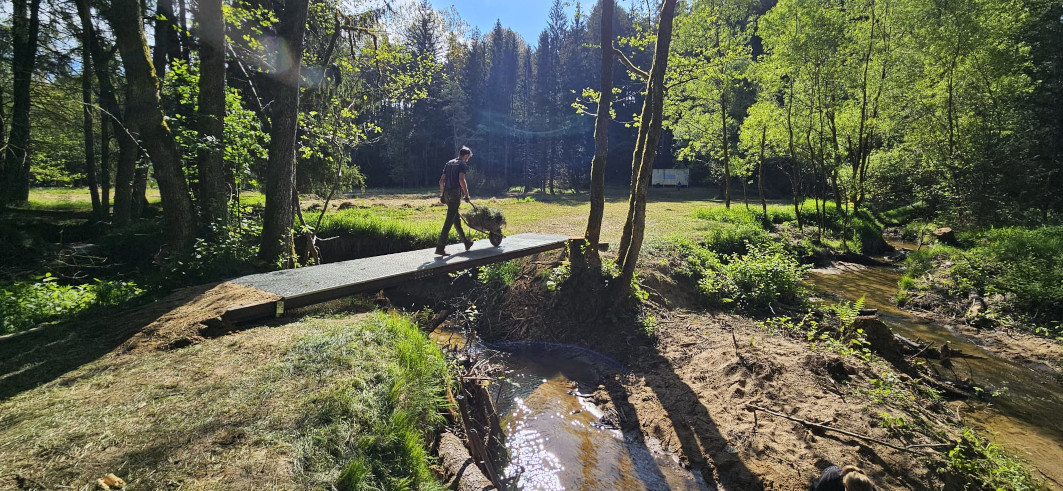
\includegraphics[width=\textwidth]{tabor-lavka.jpg}

\post{Káňata}

Cvičební rok se chýlí ke konci a stejně tak vedoucovská role Markéty,
která odchází na mateřskou dovolenou. Za všechnu oddílovou práci jí moc
děkujeme a věříme, že se s~ní budeme v~libeňském Sokole vídat i nadále.
A~protože každý konec je i novým začátkem, vítáme mezi sebou novou
vedoucí Báru, která povede oddíl od září. Prozatím probíhá činnost pod
vedením Dubiny.

Na čtvrtečních schůzkách od 15:45 hrajeme různé hry, vyrábíme a učíme
se tábornickým dovednostem. Jednou za měsíc jezdíme na výpravu. Ta
květnová směřovala ke skalním útvarům Kokořínska a první víkend v~červnu
nás čeká dvoudenní výprava do Železných hor. Vrcholem roku však bude
tábor na novém tábořišti kousek od Keblan u~Trhových Svin. Koná se od
soboty 26.7. do soboty 9.8. a ještě máme pár volných míst.

V~případě zájmu o~vstup do oddílu či jakékoliv další informace stran
Káňat, napište na e-mail
\href{mailto:jana.dubska@sokol-liben.cz}{jana.dubska@sokol-liben.cz}.

Za všechna Káňata se na nová dobrodružství těší

\signature{Jana Dubská (Dubina)}{605 959 851}

\vspace*{24pt}

\post{Oddíl žákyň}
Oddíly mladších a starších žákyň tradičně cvičí v~pondělí a čtvrtek a
dochází do nich v~průměru 20 holek na každou hodinu. I~holky se zapojily
do župních závodů všestrannosti.

2. a 5. června budou moci předškolní děti - holky přijít na
hodiny cvičení mladších žákyň, aby věděly, co je čeká za cvičení po
prázdninách.

\signature{Tomáš Dragoun}{}

\clearpage

\post{Oddíl rodičů a dětí}
Opět se nám blíží další školní rok. Hlásí se mnoho zájemců o~místa
v~oddíle, proto kdyby měl někdo chuť otevřít další hodinu cvičení rodičů
a dětí, bude tato aktivita přijata s~nadšením. Zároveň to znamená, že
kdo si nerezervuje v~systému EOS místo včas, riskuje, že v~září pro něj
žádné místo v~oddíle nebude.

Časy cvičení se nemění:

pondělí 16:00--17:00, vede Dana Cejpková

úterý 9:50--11:00, vede Jana Motlová

čtvrtek 16:00--17:00, vede Martin Kubů

Dne 26. 6. už není cvičení, protože tento den bude
zakončovací táborák, na který jste všichni zváni. Zároveň tam
poděkujeme Janě Dubské (Dubině), která už od září nepovede oddílů rodičů
a dětí.

Začínáme cvičit hned 1. 9. Přejeme krásné prázdniny.

\signature{Jana, Dana, Jana a nově Martin}{}

\post{Oddíl předškolních dětí}
Školní rok pomalu končí a některé děti už příští rok budou muset přejít
do oddílu mladších žákyň a mladších žáků.

Cvičení mladších žákyň si mohou holky vyzkoušet 2. 6. a 5. 6. od 17:00 a
kluci dne 3. 6. a 5. 6. mohou navštívit mladší žáky, kteří budou cvičit
venku.

Je potřeba si nahlásit docházku do oddílu co nejdříve, protože kdo tak
neučiní, riskuje, že od září nebude pro jeho dítě v~oddíle místo.

Hodiny zůstávají ve stejném čase:

pondělí 16:00--17:00, vede Anna Feřtová

čtvrtek 16:00--17:00, vede Dana Cejpková

Prostě jsme dobrý oddíl, což je dáno velkým množstvím cvičitelů a
pomahatelů, kteří se Vašim dětem ve svém volném čase a zdarma věnují.

Bylo by hezké, kdybychom se všichni viděli na zakončovacím táboráku dne
26. 6. (už není cvičení).

Přeji pohodové prázdniny.

\signature{Dana Cejpková}{mobil: 606 551 223\\e-mail: dana.cejpkova@sokol-liben.cz}

\post{Se Sokolem do divadla}
Určitě jste zaznamenali, že rubrika \uv{Se Sokolem do divadla}
dlouhodobě přesahuje pouhý divadelní rozměr a zahrnuje v~podstatě
veškerou kulturu a vzdělávací programy. Naše bohatá jarní nabídka a
s~kulturou/se vzděláním spojené dění to zcela jednoznačně
potvrzuje\ldots{}

\subpost{Rozesílací seznam}
Dříve než Vás seznámím, co je nového na poli
kultury, dovolím si připomenout existenci \uv{rozesílacího seznamu} pro
kulturychtivé jedince. Některé nabídky na představení je totiž potřeba
řešit velmi rychle, ať už z~důvodu nemožnosti rezervace nebo dostupnosti
vstupenek. Máte-li zájem, rád vás zařadím do již existujícího
rozesílacího seznamu -- stačí, když mi svůj zájem oznámíte e-mailem
(\href{mailto:mila.doupal@sokol-liben.cz}{\nolinkurl{mila.doupal@sokol-liben.cz}}).
Díky rozesílacímu seznamu obdržíte nabídku na kulturní akci jako první
bez prodlevy zveřejnění v~klubové platformě EOS -- hlavně se dozvíte i
o~akcích (organizovaných i neorganizovaných), které se v~EOSu z~výše
uvedených důvodů ani neobjeví. Budete tak mít jistotu, že se o~všech
akcích konaných v~rámci projektu \uv{SE SOKOLEM DO DIVADLA} dozvíte včas.

\subpost{Stalo se}
Se zimou jsme se rozloučili 20. března 2025
v~Rudolfinu za zvuků posledního koncertu vzdělávacího cyklu, který byl
věnován Modestu Petroviči Musorgskému a jeho Obrázkům z~výstavy.
O~vtipný a poučný komentář se postarali jako vždy dirigent Marko Ivanović
a moderátor Petr Kadlec. Ve vyprodaném Rudolfinu obsadil Sokol Libeň
celkem 11 míst.

Jarní kulturní turné jsme zahájili 11. dubna 2025 vtipným představením
v~Divadle v~Dlouhé. Součástí komedie \uv{Tajný deník Adriana Molea ve věku
13 a ¾} byly nejen herecké výkony plné typických projevů a znaků
pubertálního chování, ale i živá hudba s~podobně laděnými texty. Nabídky
využilo 24 osob.

Jako další v~řadě proběhla 24. dubna 2025 premiéra dokumentárního filmu
\uv{Pohřbené naděje} z~dílny organizace Gulag.cz, která sídlí v~prostorách
naší sokolovny. V~kině Aero sledovali 3 zájemci z~našich řad jejich
pátrání po českých stopách v~Kyrgyzstánu, kde by je, přiznejme si to,
hledal asi málokdo\ldots{} Film doporučuji ke shlédnutí i mimo premiéru.

Zmíněný rozesílací seznam splnil svou úlohu ve chvíli, kdy jsme obdrželi
\uv{last minute} nabídku z~Divadla v~Dlouhé za lákavých 150 Kč. Dne 6.
května 2025 jsme zhlédli představení \uv{Pravomil} vyprávějící očima
osvědčeného režiséra Tomáše Dianišky pohnutý životní příběh Pravomila
Raichla s~plnohodnotnou dějinnou kulisou. I~když za Libeň se zúčastnilo
celkem 8 dospělých, divadlo bylo plné studentů, kteří tak mohli zasadit
teoretické znalosti z~dějepisu do konkrétnějšího životního rámce.

V~podobném duchu se neslo i představení \uv{294 statečných}, které
v~Divadle pod Palmovkou navštívilo v~měsíc výročí splnění operace
Anthropoid celkem 21 zájemců. I~tato emotivně silná adaptace příběhu
pochází z~pera oceňovaného Tomáše Dianišky.

\subpost{Co nás čeká}
Rozesílací seznam posloužil i pro nabídku
z~jiného \uv{soudku}, které využilo 9 zájemců. V~Divadle Bravo nás 26.
května 2025 čeká akrobaticko-taneční novocirkusové vystoupení s~názvem
\uv{The Losers}.

Tento školní rok bychom pak zakončili absolventským koncertem libeňského
Jilmáka Daniela Kadlece (Daněk). Společně s~naším dirigentem, který si
bude taktovku střídat se svou profesorkou Miriam Němcovou, se představí
Filharmonie Hradec Králové a několik sólistů. Koncert se uskuteční na
Pražské konzervatoři dne 12. června 2025. Bližší informace budeme sdílet
co nejdříve. Vstup na koncert je volný.

Svou premiéru rozesílací seznam zaznamenal ku příležitosti omezené
nabídky na představení \uv{Audience pro královnu}, které se bude ve
Stavovském divadle konat poslední den prázdnin 31. srpna 2025. Že se
jedná o~mimořádnou nabídku, dosvědčuje skutečnost, že se přihlásilo ve
velmi krátkém čase celkem 26 zájemců, čímž jsme plně využili naši časově
a kapacitně limitovanou rezervaci.

Do 11. května 2025 probíhala aktuálně poslední nabídka týkající se
dalšího ročníku série vzdělávacích pořadů v~Rudolfinu, které se v~další
sezóně ponesou v~duchu koncertů \uv{Na přání\ldots}:


\begin{itemize}[
  itemsep=-3pt,
  leftmargin=1em,
  itemindent=-1em
]
\item[] 24. října 2025 se bude hrát \uv{na přání orchestru}
\item[] 6. března 2026 své přání odhalí \uv{sólista}
\item[] 29. dubna 2026 nám svá přání představí dirigent Marko Ivanović
\end{itemize}

Na nový ročník se těší minimálně 13 zájemců, kteří si předplatili celé
abonmá zahrnující celkem 3 vzdělávací koncerty.

Pokud by se našel ještě nějaký dodatečný zájemce, ozvěte se mi co
nejdříve a pokusil bych se dojednat v~rámci kapacity sálu nějaká volná
místa na samostatné koncerty nebo celé abonmá.

\subpost{Nabídky odjinud\ldots{}}
Krom našich interních akcí a nabídek
mohu s~radostí sdílet i tipy a nabídky sokolského projektu \uv{Do Sokola za
kulturou}, který má na starosti sestra Jarka Knížková. Připravované
akce byste měli najít na
\href{https://prosokoly.sokol.eu/kultura-v-tyrsove-dome}{\emph{https://prosokoly.sokol.eu/kultura-v-tyrsove-dome}};
z~nejbližších vybírám:

\begin{itemize}[
  itemsep=-3pt,
  leftmargin=1em,
  itemindent=-1em
]
  \item[] Michnův palác: 10. 6. 2025 od 19,00 h – Koncert swingové formace Modrá synkopa
  \item[] Michnův palác: 11. 6. 2025 od 19,00 h – Anička Jagošová – cimbálovka a Dětský pěvecký sbor Dany Ungrové
\end{itemize}

\noindent
\emph{Pozn: Uvedené sokolské tipy jen přeposílám a upozorňuji, že ve
výjimečných případech se může stát, že dojde ke změně data nebo místa
konání. Bližší informace naleznete zde:
\href{https://prosokoly.sokol.eu/kultura-v-tyrsove-dome}{https://prosokoly.sokol.eu/kultura-v-tyrsove-dome}.
Vstupné, většinou symbolické, je hrazeno těsně před vstupem na akci.}

\subpost{Novinka – Akademie věd}
Rád bych Vás seznámil s~poslední,
spíše vzdělavatelskou než kulturní, novinkou. Sokol Libeň bude od června
2025 dostávat výtisky periodik vydávaných Akademií věd ČR. I~když jsou
texty většinou laděny odborněji, jsou psané srozumitelně a věřím, že
mnoho zvídavých sokolíků v~nich najde zajímavé informace ze světa
české vědy a akademického prostředí. Budeme mít standardně
k~dispozici celkem 10 výtisků -- ty budou volně k~rozebrání na vrátnici,
případně budou rozmístěny na stolech jako četba \uv{pro volné chvíle} --
např. pro čekající cvičence nebo doprovod mladších cvičenců. Po přečtení
můžete i starší čísla vrátit k~vrátnici pro další případné zájemce --
informace obsažené ve výtiscích totiž hned tak nezestárnou a budou
aktuální i dlouho po jejich prvním vydání\ldots{}

Dal jsem si interní cimrmanovské předsevzetí do konce školního roku
2024/2025 \uv{nic dalšího nerozjíždět}, ale \uv{jeden} nikdy neví\ldots{}
Těch zajímavých tipů a nabídek je totiž tolik, že se třeba \uv{jeden}
neudrží a zas něco pošle\ldots{}

A~pokud byste měl někdo jiný zajímavý tip, klidně jej nasdílejte na níže
uvedený e-mail.

Nejen pohybu, ale i kultuře a hlavně vzdělání -- ZDAR!

\signature{Miloslav Doupal}{e-mail: mila.doupal@sokol-liben.cz}

\post{Šibřinky}
8. března odpoledne a večer jsme uspořádali pro naše členy a přátele
tradiční Šibřinky. Letošním tématem byl cirkus, což inspirovalo k~řadě
kostýmů a masek. Do soutěže masek se přihlásilo celkem 20 soutěžících
jednotlivců, dvojic i skupin. A~právě dvojice Liška a Kondor se svojí
maskou Provazochodkyně a provaz v~soutěži zvítězili, když ji jako
nejlepší vyhodnotilo 24 hlasujících z~celkového počtu 88 hlasujících. Na
druhém místě se umístili tradičně vysoko bodující Hanka a Míla
Doupalovi. Třetí místo v~soutěži masek obsadila Mráťa hlavně díky
kontinuální kampani v~průběhu večera a množství rozdaných nafukovacích
pejsků.

Celým večerem nás doprovázela hudba skupiny Kdo má čas a v~průběhu
večera pro nás vystoupili sestry a bratři se sokolskou besedou,
akrojógou a irskými tanci. Celkem bylo návštěvníků Šibřinek 110. Na
všechny, kteří se rozhodli pro zakoupení tombolového kolíčku, čekala
menší či větší odměna, a to díky řadě drobnějších darů od členů naší
jednoty, ale i hodnotnějších cen z~řad našich podporovatelů a přátel
z~blízkého i vzdálenějšího okolí. Již nyní se těšíme na další téma a
přátelský společenský večer v~roce 2026.

\signature{Tomáš Dragoun}{organizátor}

\begin{center}
\includegraphics[width=0.96\textwidth]{sibrinky.JPG}
\end{center}

\clearpage
\post{Sokolská kapka krve}

Projekt pokračuje od ledna t. r. 11. ročníkem. V~letošním roce nastala
malá organizační změna, kdy se budou nahlašovat počty odběrů pouze
jednou za celý rok, za ten letošní do 31. 1. 2026.

V~době letních prázdnin bývá odběrů méně, zejm. z~důvodů dovolených.
Proto pokud můžete, zkuste si svůj odběr naplánovat právě na tuto dobu.

Podrobnosti i za uplynulé ročníky nebo další informace lze dohledat na
\href{http://www.sokolsakapkakrve.cz}{www.sokolskakapkakrve.cz},
případně je rád sdělím osobně či na e-mailu
\href{mailto:vit.jakoubek@sokol-liben.cz}{vit.jakoubek@sokol-liben.cz}.

A nezapomeňte: 14.6. si připomínáme Mezinárodní den dárců krve!

\signature{Vít Jakoubek}{koordinátor projektu}
\vspace*{24pt}

\begin{center}
  
\includegraphics[width=0.5\textwidth]{./sokolska_kapka_krve.jpg}
  \end{center}
  

% zadní obálka
\clearpage

\pagestyle{blank}
\newgeometry{margin=1cm}

\vspace*{96pt}

\pagecolor{sokolred}
\color{white}

\noindent {\fontsize{48pt}{56pt}\tyrs
se sokolským

\vspace*{24pt}

\noindent nazdar!}

\vspace*{\fill}

% \color{black}
\begin{center}
Vydává Tělocvičná jednota Sokol Libeň, Zenklova 37, Praha 8

\vspace*{12pt}

Na přípravě tohoto čísla se spolu s~autory jednotlivých textů podíleli:

grafická úprava – Martin Burian | jazyková úprava – Martina Waclawičová \\ editoři textů – Vít Jakoubek, Jan Přech
\end{center}

\end{document}